%%%% Modelo de estados de Entidades del sistema.
El presente capítulo describe el modelo de estados correspondiente a las entidades del Calmécac que tienen un comportamiento dinámico en el sistema. Está conformado por los siguientes elementos:
\begin{itemize}
	\item Modelo del ciclo de vida de la \refElem{EstructuraEducativa} de una \refElem{UnidadAcademica} en la sección \refElem{sec:SM-EE}, el cual describe la evolución de la Estructura Educativa desde que es creada hasta que es cerrada cuando termina el periodo para el que fue definida.
	
	\item Modelo del ciclo de vida de un elemento de la \refElem{EstructuraEducativa} en la sección \refElem{sec:SM-ElementoEE}, el cual describe la evolución de un elemento de la Estructura Educativa desde que es creado hasta que es aprobada o se le realizan cambios una vez que ha sido aprobada.
\end{itemize}

%% Máquina de estados general de la Estructura Educativa
\begin{Maquina}{sec:SM-EE}{Modelo del ciclo de vida de la Estructura Educativa de una Unidad Académica}{
En cualquier momento dado, la \refElem{tEstructuraEducativa} de una \refElem{tUnidadAcademica} correspondiente a un \refElem{tPeriodoEscolar} y a una \refElem{tModalidad} tiene un 'estado' en el sistema. Las acciones que los actores pueden realizar sobre la Estructura Educativa dependen de dicho estado y pueden tener como consecuencia la transición a otro. Un resumen de las acciones posibles sobre la Estructura Educativa dependiendo del estado se muestran en la Tabla \ref{SM:estadosEE}. 

Los actores involucrados en el ciclo de vida de la Estructura Educativa son:
\begin{itemize} 
	\item \refElem{UAParticipanteEE}: Este actor engloba a todos los participantes de la definición de la Estructura Educativa dentro de la Unidad Académica. Cuando existen funciones que son particulares a un actor específico, se indican de forma separada para dicho actor como es el caso del \refElem{UAResponsableEstructuraEducativa}.
	\item \refElem{DESAnalista}
	\item \refElem{DESResponsableEE}
\end{itemize}
 

Los estados y transiciones posibles del ciclo de vida de la Estructura Educativa se muestran en la Figura \ref{fig:sec:SM-EE} y se describen a continuación.	
}{images/maquinasEstados/EstructuraEducativa.png}
%\begin{figure}[htbp!]
%	\centering
%	\fbox{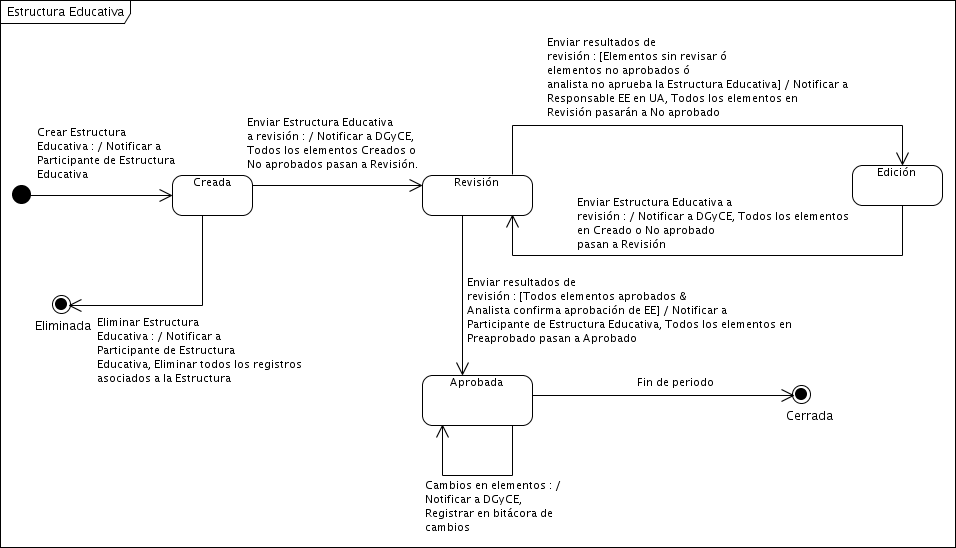
\includegraphics[width=\textwidth]{images/maquinasEstados/EstructuraEducativa.png}}
%	\caption{Modelo del ciclo de vida de la Estructura Educativa}
%	\label{fig:maquinaEstadosEE}
%\end{figure}

\begin{description}

% ESTADO: Creada
\item[Creada:] Este es el estado con el que inicia la Estructura Educativa después de que ha sido creada, ya sea en blanco o como copia de la Estructura Educativa de algún periodo anterior. Cuando la Estructura Educativa es creada, se notifica de su creación a los participantes de la misma ( ver \refElem{UAParticipanteEE} ). Estar en este estado significa que los componentes de la Estructura están siendo gestionados por parte del \refElem{UAParticipanteEE} y que la Estructura Educativa acaba de ser creada y no ha sido enviada para Revisión de la DGyCE. Para la Estructura estar en este estado implica que:

\begin{description}
	\item[\refElem{UAParticipanteEE}:] Este actor puede:
	\begin{itemize} 
		\item Modificar los elementos que la conforman de acuerdo con el estado del elemento.
		\item Modificar los horarios asociados con elementos creados.
		\item Consultar los elementos que la conforman.
		\item Añadir elementos.
		\item Eliminar elementos que la conforman.
	\end{itemize}
	
	
	\item[\refElem{UAResponsableEstructuraEducativa}:] Este actor puede:
	\begin{itemize} 
%		\item Cambiar su configuración.
		
		\item Enviarla para revisión, resultando en la transición hacia el estado {\bf Revisión}, la transición hacia el estado {\bf Revisión} de todos los elementos que no han sido aprobados y el envío de una notificación al \refElem{DESAnalista} y \refElem{DESResponsableEE} indicando que existen elementos de la Estructura Educativa listos para revisión.
		
		\item Eliminarla, resultando en la transición hacia el estado {\bf Eliminada} y el envío de una notificación a cada \refIdElem{UAParticipanteEE} indicándole que la Estructura Educativa ha sido eliminada.
	\end{itemize}	
	
	\item[\refElem{DESAnalista}:] Este actor no tiene acceso a la Estructura Educativa.
	
	\item[\refElem{DESResponsableEE}:] Este actor no tiene acceso a la Estructura Educativa.
	
\end{description}

% ESTADO: Revisión
\item[Revisión:] En este estado la Estructura Educativa está siendo revisada por \refElem{DESAnalista} o \refElem{DESResponsableEE} quienes pueden determinar si aprueban o no cada elemento de forma independiente. En este estado no se permite la modificación de horarios asociados a los elementos en revisión. Para la Estructura Educativa, estar en este estado implica que:%Al terminar la revisión de todos los elementos que se encuentran en estado {\bf Revisión}, se da pie a dos posibles transiciones:
%\begin{itemize} 
%	\item Hacia el estado {\bf Edición} si existe al menos un elemento cuyo estado no es {\bf Aprobado} o, ya sea el \refElem{DESAnalista} o el \refElem{DESResponsableEE}, no confirma la aprobación de la Estructura. Esto causa que todos los elementos que se encontraban en {\bf Revisión} cambien de estado a {\bf Edición} y se le notifique al \refElem{UAResponsableEstructuraEducativa} que la Estructura Educativa no ha sido aprobada.
%	
%	\item Hacia el estado {\bf Aprobada} si todos los elementos existentes han sido aprobados y el \refElem{DESAnalista} o \refElem{DESResponsableEE} confirman la aprobación de la Estructura. Cuando esto ocurre, se le notifica al \refElem{UAResponsableEstructuraEducativa} la aprobación de la Estructura Educativa.
%\end{itemize}


\begin{description}
	\item[\refElem{UAParticipanteEE}:] Este actor puede:% consultar los elementos que la conforman.
	\begin{itemize} 
		\item Modificar los elementos que la conforman de acuerdo con el estado del elemento.
		\item Consultar los elementos que la conforman.
		\item Añadir elementos.
		\item Modificar los horarios asociados con elementos creados.
		\item Eliminar elementos de acuerdo con el estado del elemento.
	\end{itemize}
	
	\item[\refElem{DESAnalista}:] Este actor puede:
	\begin{itemize} 
		\item Consultar los elementos que la conforman.
		\item Revisar los elementos, lo que puede tener dos posibles resultados: aprobarlos o no.
		\item Realizar observaciones sobre los elementos.
		\item Enviar a la Unidad Académica los resultados de la revisión, lo que da pie a dos posibles transiciones:
		\begin{itemize} 
			\item Hacia el estado {\bf No aprobada} si existen elementos sin revisar (en estado {\bf Revisión}), elementos cuyo estado es {\bf No Aprobado} o, ya sea el \refElem{DESAnalista} o el \refElem{DESResponsableEE}, no aprueban la Estructura. Esto causa que todos los elementos que se encontraban en {\bf Revisión} cambien de estado a {\bf No aprobado} y se le notifique al \refElem{UAResponsableEstructuraEducativa} que la Estructura Educativa no ha sido aprobada.
			
			\item Hacia el estado {\bf Aprobada} si todos los elementos existentes han sido aprobados y el \refElem{DESAnalista} o \refElem{DESResponsableEE} aprueba la Estructura. Cuando esto ocurre, se le notifica al \refElem{UAResponsableEstructuraEducativa} la aprobación de la Estructura Educativa.
		\end{itemize}
	\end{itemize}
	
	\item[\refElem{DESResponsableEE}:] Este actor puede:
	\begin{itemize} 
		\item Consultar los elementos que la conforman.
		\item Revisar los elementos, lo que puede tener dos posibles resultados: aprobarlos o no.
		\item Realizar observaciones sobre los elementos.
		\item Enviar a la Unidad Académica los resultados de la revisión, lo que da pie a dos posibles transiciones:
		\begin{itemize} 
			\item Hacia el estado {\bf No aprobada} si existen elementos sin revisar (en estado {\bf Revisión}), elementos cuyo estado es {\bf No Aprobado} o, ya sea el \refElem{DESAnalista} o el \refElem{DESResponsableEE}, no aprueban la Estructura. Esto causa que todos los elementos que se encontraban en {\bf Revisión} cambien de estado a {\bf No aprobado} y se le notifique al \refElem{UAResponsableEstructuraEducativa} que la Estructura Educativa no ha sido aprobada.
			
			\item Hacia el estado {\bf Aprobada} si todos los elementos existentes han sido aprobados y el \refElem{DESAnalista} o \refElem{DESResponsableEE} aprueba la Estructura. Cuando esto ocurre, se le notifica al \refElem{UAResponsableEstructuraEducativa} la aprobación de la Estructura Educativa.
		\end{itemize}
	\end{itemize}
\end{description}



% ESTADO: No aprobada
\item[No aprobada:] Este es el estado en el que se encuentra la Estructura Educativa después de que ha sido revisada y no fue aprobada, ya sea debiado a que existen elementos creados o no aprobados (ver \refElem{sec:SM-ElementoEE} ) o el \refElem{DESAnalista} no la ha aprobado. Estar en este estado significa que los componentes de la Estructura están siendo gestionados por parte del \refElem{UAParticipanteEE}. Para la Estructura estar en estado implica que:

\begin{description}
	\item[\refElem{UAParticipanteEE}:] Este actor puede:
		\begin{itemize} 
			\item Modificar los elementos que la conforman de acuerdo con el estado del elemento.
			\item Consultar los elementos que la conforman.
			\item Modificar los horarios asociados con los elementos.
			\item Añadir elementos.
			\item Eliminar elementos de acuerdo con el estado del elemento.
		\end{itemize}

	\item[\refElem{UAResponsableEstructuraEducativa}:] Este actor puede enviarla para revisión, resultando en la transición hacia el estado {\bf Revisión}, la transición hacia el estado {\bf Revisión} de todos los elementos que no han sido aprobados y el envío de una notificación al \refElem{DESAnalista} y \refElem{DESResponsableEE} indicando que existen elementos de la Estructura Educativa listos para revisión. 
		
	
	\item[\refElem{DESAnalista}:] Este actor puede consultar los elementos que han sido aprobados previamente.
			
	\item[\refElem{DESResponsableEE}:] Este actor puede consultar los elementos que han sido aprobados previamente.
	
\end{description}

% ESTADO: Aprobada
\item[Aprobada:] En este estado la Estructura Educativa ha sido aprobada por la DGyCE. Se pueden realizar cambios en la Estructura los cuales quedarán registrados en la bitácora de cambios y producen una transición a este mismo estado. Es posible agregar o eliminar elementos y estas acciones también quedarán registrados en la bitácora de cambios. Es partir de este estado que la Estructura Educativa puede ser copiada para servir de base a Estructuras Educativas futuras. Para la estructura estar en este estado implica que:
	\begin{description}
		\item[\refElem{UAParticipanteEE}:] Este actor puede:
		\begin{itemize} 
			\item Modificar los elementos que la conforman de acuerdo con el estado del elemento.
			\item Consultar los elementos que la conforman.
			\item Añadir elementos.
			\item Modificar los horarios asociados con los elementos.
			\item Eliminar elementos de acuerdo con el estado del elemento.
		\end{itemize}
		
		\item[\refElem{DESAnalista}:] Este actor puede consultar los elementos que ya han sido aprobados.
		
		\item[\refElem{DESResponsableEE}:] Este actor puede consultar los elementos que ya han sido aproabdos.
	\end{description}

% ESTADO: Cerrada
\item[Cerrada:] Este es el estado al que pasa la Estructura Educativa una vez que el periodo para el que fue definida concluye. En este estado todos los actores involucrados pueden consultar sus elementos pero no se admite ningún tipo de modificación. 

% ESTADO: Eliminada
\item[Eliminada:] Este estado indica que la Estructura Educativa ha sido eliminada del sistema y por lo tanto ningún actor puede realizar operación alguna sobre ella. Cuando esto ocurre, todos los elementos de la Estructura también se eliminan.

\end{description}


\begin{longtable}{| p{0.35\textwidth} | p{0.6\textwidth} |}
	\hline  
	\label{SM:estadosEE} 
	{\bf Estado de Estructura Educativa}  & {\bf Acciones sobre Estructura Educativa}\\
	\endfirsthead
	\hline
	Creada & 
	\begin{Titemize} 
		\Titem Agregar elementos.
		\Titem Modificar los horarios asociados con elementos.
		\Titem Editar elementos
		\Titem Eliminar elementos
		\Titem Consultar elementos
		\Titem Enviarla a revisión
		\Titem Eliminarla
%		\Titem Realizar observaciones sobre los elementos
%		\Titem Revisar elementos
%		\Titem Enviar resultados de revisión
	\end{Titemize}\\ 
	\hline
	Revisión &  
	\begin{Titemize} 
		\Titem Agregar elementos.
		\Titem Modificar los horarios asociados con elementos que no se encuentren en revisión.
		\Titem Editar elementos que no se encuentren en revisión.
		\Titem Eliminar elementos que no se encuentren en revisión.
		\Titem Consultar elementos
		\Titem Realizar observaciones sobre los elementos
		\Titem Revisar elementos
		\Titem Enviar resultados de revisión
	\end{Titemize}\\ 
	\hline
	No Aprobada & 
	\begin{Titemize} 
		\Titem Agregar elementos.
		\Titem Modificar los horarios asociados con elementos.
		\Titem Editar elementos
		\Titem Eliminar elementos
		\Titem Consultar elementos
		\Titem Enviarla a revisión
	\end{Titemize}\\
	\hline
	Aprobada & 
	\begin{Titemize} 
		\Titem Agregar elementos.
		\Titem Modificar los horarios asociados con elementos.
		\Titem Editar elementos
		\Titem Eliminar elementos
		\Titem Consultar elementos
		\Titem Realizar una copia para una Estructura Educativa futura.
	\end{Titemize}\\ 
	\hline
	Cerrada  & 
	\begin{Titemize} 
		\Titem Consultar elementos
		\Titem Realizar una copia para una Estructura Educativa futura.
	\end{Titemize}\\ 
	\hline
	Eliminada & Ninguna\\ 
	\hline
	\caption{Acciones que se pueden realizar sobre una Estructura Educativa dependiendo de su estado}
\end{longtable}
\end{Maquina}

%% Máquina de estados de un elemento de la Estructura Educativa
\begin{Maquina}{sec:SM-ElementoEE}{Modelo del ciclo de vida de un Elemento de la Estructura Educativa de una Unidad Académica} {
En cualquier momento dado, un elemento de la \refElem{tEstructuraEducativa} de una \refElem{tUnidadAcademica} correspondiente a un \refElem{tPeriodo} y a una \refElem{tModalidad} tiene un 'estado' en el sistema. Las acciones que los actores pueden realizar sobre el elemento dependen de dicho estado y del estado de la Estructura Educativa a la que pertenece ( ver \refElem{sec:SM-EE} ) y pueden tener como consecuencia la transición a otro. Las posibles combinaciones de estados entre ambas máquinas y las acciones posibles sobre los elementos se muestran en la Tabla \ref{SM:combinatoriaEstados}.

Los actores involucrados en el ciclo de vida de un Elemento de la Estructura Educativa son:
\begin{itemize} 
	\item \refElem{UAParticipanteEE}: Este actor engloba a todos los que participan en la definición de la Estructura Educativa dentro de la Unidad Académica. Cuando existen funciones que son particulares a un actor específico, se indican de forma separada para dicho actor.
	\item \refElem{DESAnalista}
	\item \refElem{DESResponsableEE}
\end{itemize}

Los estados y transiciones posibles del ciclo de vida de un Elemento de la Estructura Educativa se muestran en la figura \ref{fig:sec:SM-ElementoEE} y se describen a continuación.	
%
%\begin{figure}[htbp!]
%	\centering
%	\fbox{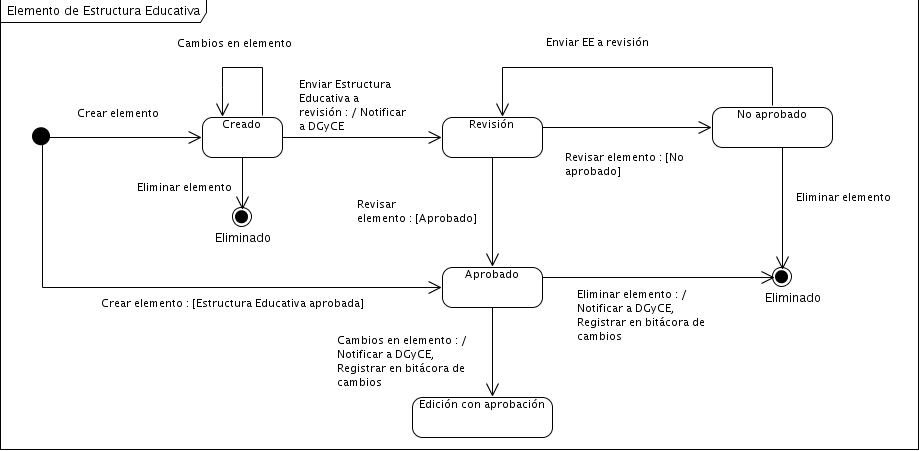
\includegraphics[width=\textwidth]{images/maquinasEstados/ElementoEstructuraEducativa.png}}
%	\caption{Modelo del ciclo de vida de un Elemento de la Estructura Educativa}
%	\label{fig:maquinaEstadosElementoEE}
%\end{figure}
}{images/maquinasEstados/ElementoEstructuraEducativa.png}
\begin{description}

% ESTADO: Edición
\item[Creado:] Este es el estado en el que comienza el elemento de la Estructura Educativa una vez que ha sido creado y la Estructura Educativa a la que pertenece no ha sido aprobada. El elemento pudo haber sido fue agregado o copiado de una Estructura Educativa de un periodo anterior. Estar en este estado significa que el elemento está siendo editado por el \refElem{UAParticipanteEE}. Existen dos posibles transiciones que salen de este estado:
\begin{itemize} 
	\item Hacia el estado {\bf Revisión} cuando la Estructura Educativa a la que pertenece es enviada a revisión
	\item Hacia este estado cuando se realizan cambios en el elemento.
\end{itemize}

Para el elemento, estar en este estado implica que:
	\begin{description}
		\item[\refElem{UAParticipanteEE}:] Este actor puede:
		\begin{itemize} 
			\item Editarlo
			\item Eliminarlo, resultando en una transición hacia el estado {\bf Eliminado}.
			\item Consultarlo
			\item Enviarlo a revisión
			\item Modificar los horarios a los que está asociado.
			%\item Revisarlo
			%\item Hacerle observaciones
		\end{itemize}
	
		\item[\refElem{DESAnalista}:] Este actor no tiene acceso al elemento.
		
		\item[\refElem{DESResponsableEE}:] Este actor no tiene acceso al elemento.
	\end{description}

% ESTADO: Revisión
\item[Revisión:] El elemento pasa a este estado cuando la Estructura Educativa es enviada a revisión (ver \refElem{sec:SM-EE}) y significa que está siendo revisado por \refElem{DESAnalista} o \refElem{DESResponsableEE}. Para el elemento, estar en estado implica que:
	\begin{description}
		\item[\refElem{UAParticipanteEE}:] Este actor puede consultarlo.
		
		\item[\refElem{DESAnalista}:] Este actor puede:
		\begin{itemize} 
			\item Consultarlo.
			\item Hacerle observaciones
			\item Revisarlo, dando pie a dos transiciones posibles:
			\begin{itemize} 
				\item Hacia el estado {\bf No aprobada} en caso de que no apruebe el elemento, lo que produce el envío de una notificación al \refElem{UAResponsableEstructuraEducativa} indicándole que el elemento no ha sido aprobado.
				\item Hacia el estado {\bf Aprobado} en caso de que apruebe el elemento.
			\end{itemize}
		\end{itemize}
	
		\item[\refElem{DESResponsableEE}:] Este actor puede:
		\begin{itemize} 
			\item Consultarlo.
			\item Hacerle observaciones
			\item Revisarlo, dando pie a dos transiciones posibles:
			\begin{itemize} 
				\item Hacia el estado {\bf No aprobada} en caso de que no apruebe el elemento, lo que produce el envío de una notificación al \refElem{UAResponsableEstructuraEducativa} indicándole que el elemento no ha sido aprobado.
				\item Hacia el estado {\bf Aprobado} en caso de que apruebe el elemento.
			\end{itemize}
		\end{itemize}
	
	\end{description}

% ESTADO: Preaprobado
%\item[Preaprobado:] En este estado el elemento de la Estructura Educativa ha sido aprobado pero la Estructura Educativa a la que pertenece no. En este estado se pueden realizar cambios en el elemento sin que estos se reflejen en la bitácora o eliminarlo en caso de que sea necesario. Cuando la Estructura Educativa a la que pertenece el elemento es aprobada, todos los elementos que se encuentren en este estado pasan a {\bf Aprobado}. Para el elemento, estar en este estado implica que:
%\begin{description}
%	\item[\refElem{UAParticipanteEE}:] Este actor puede:
%	\begin{itemize} 
%		\item Consultarlo
%		\item Eliminarlo, siempre y cuando la Estructura Educativa a la que pertenece esté en {\bf Edición}, resultando en una transición hacia el estado {\bf Eliminado}
%		\item Modificarlo, siempre y cuando la Estructura Educativa a la que pertenece esté en {\bf Edición}, resultando en una transición hacia el estado {\bf Edición}.
%	\end{itemize}
%	
%	\item[\refElem{DESAnalista}:] Este actor puede consultarlo.
%	
%	\item[\refElem{DESResponsableEE}:] Este actor puede consultarlo.	
%	
%\end{description}


% ESTADO: Aprobado
\item[Aprobado:] El elemento pasa a este estado cuando el resultado de su revisón es aprobado o cuando la Estructura Educativa está aprobada al momento de su creación. Se pueden realizar cambios al elemento en este estado considerando que todo cambio que se haga se registra en la bitácora de cambios. Para el elemento, estar en este estado implica que:
	\begin{description}
		\item[\refElem{UAParticipanteEE}:] Este actor puede:
		\begin{itemize} 
			\item Editarlo, resultando en el envío de una notificación al \refElem{DESAnalista} indicándole del cambio.
			\item Eliminarlo, resultando en una transición hacia el estado {\bf Eliminado}, el registro de la eliminación en la bitácora de cambios y el envío de una notificación al \refElem{DESAnalista} indicándole de la eliminación
			\item Consultarlo 
			\item Modificar los horarios a los que está asociado.
		\end{itemize}
	
		\item[\refElem{DESAnalista}:] Este actor puede consultarlo.

		\item[\refElem{DESResponsableEE}:] Este actor puede consultarlo.	
	
	\end{description}
	
% ESTADO: Edición con aprobación	
\item[Edición con aprobación:] Estar en este estado significa que el elemento ha sido modificado después de haber sido aprobado. Para el elemento, estar en este estado implica que:
	\begin{description}
		\item[\refElem{UAParticipanteEE}:] Este actor puede:
		\begin{itemize} 
			\item Editarlo, resultando en el envío de una notificación al \refElem{DESAnalista} indicándole del cambio.
			\item Eliminarlo, resultando en una transición hacia el estado {\bf Eliminado}, el registro de la eliminación en la bitácora de cambios y el envío de una notificación al \refElem{DESAnalista} indicándole de la eliminación
			\item Consultarlo 
			\item Modificar los horarios a los que está asociado.
		\end{itemize}
		
		\item[\refElem{DESAnalista}:] Este actor puede consultarlo.
		
		\item[\refElem{DESResponsableEE}:] Este actor puede consultarlo.

	\end{description}

%ESTADO: Eliminado
\item[Eliminado:] Este estado indica que el Elemento de la Estructura Educativa ha sido eliminado del sistema y por lo tanto ningún actor puede realizar operación alguna sobre él.

\end{description}

\begin{longtable}{| p{.12\textwidth} | p{.12\textwidth} | p{.06\textwidth}| p{.07\textwidth}| p{.1\textwidth}| p{.1\textwidth}| p{.1\textwidth}| p{.1\textwidth}| p{.1\textwidth}| }
	\hline  
	\rowcolor{colorPrincipal}
	\multicolumn{9}{|c|}{\bf\color{white}{Tabla de Estados}}\\\hline
	\label{SM:combinatoriaEstados} 
	{\bf Estado de Estructura Educativa} & {\bf Estado de Elemento de Estructura Educativa} & {\bf Editar} & {\bf Eliminar} & {\bf Consultar} & {\bf Enviar a revisión}  & {\bf Modificar horarios asociados} & {\bf Revisar} & {\bf Hacer observaciones}\\
	\endfirsthead
%	\hline\multicolumn{1}{|c|}{\textbf{Estado de Estructura Educativa}} &
%	\multicolumn{1}{|c|}{\textbf{Estado de Elemento de Estructura Educativa}} &
%	\multicolumn{1}{c|}{\textbf{Acciones sobre elemento}} \\ \hline 
%	\endhead
	\hline
	Creada & Creado & Sí & Sí & Sí & Sí  & Sí & No & No\\
	\hline
	Creada & Revisión & \multicolumn{7}{c|}{No válido}\\
	\hline
	Creada & No aprobado & \multicolumn{7}{c|}{No válido}\\
	\hline
	Creada & Aprobado & \multicolumn{7}{c|}{No válido}\\
	\hline
	Creada & Edición con aprobación & \multicolumn{7}{c|}{No válido}\\
	\hline
	Revisión & Creado & Sí & Sí & Sí & No & Sí & No & No\\
	\hline
	Revisión & Revisión & No & No & Sí & No & No & Sí & Sí\\
	\hline
	Revisión & No aprobado & No & No & Sí & No & No & No & No\\
	\hline
	Revisión & Aprobado & No & No & Sí & No & No & No & No\\
	\hline
	Revisión & Edición con aprobación & No & No & Sí & No & No & No & No\\
	\hline
	No aprobada & Creado & Sí & Sí & Sí & No & Sí & No & No\\
	\hline
	No aprobada & Revisión & \multicolumn{7}{c|}{No válido}\\
	\hline
	No aprobada & No aprobado & Sí & Sí & Sí & No & Sí & No & No\\
	\hline
	No aprobada & Aprobado & Sí & Sí & Sí & No & Sí & No & No\\
	\hline
	No aprobada & Edición con aprobación & Sí & Sí & Sí & No & Sí & No & No\\
	\hline
	Aprobada & Creado & \multicolumn{7}{c|}{No válido}\\
	\hline
	Aprobada & Revisión & \multicolumn{7}{c|}{No válido}\\
	\hline
	Aprobada & No aprobado & \multicolumn{7}{c|}{No válido}\\
	\hline
	Aprobada & Aprobado & Sí & Sí & Sí & No & Sí & No & No\\
	\hline
	Aprobada & Edición con aprobación & Sí & Sí & Sí & No & Sí & No & No\\
	\hline
	Cerrada & Cualquiera & No & No & Sí & No & No & No & No\\
	\hline
	\caption{Combinaciones posibles de estados del ciclo de vida de una Estructura Educativa y un Elemento de la Estructura Educativa y acciones posibles sobre el elemento.}
\end{longtable}

\end{Maquina}